\documentclass[12pt,a4paper]{article}

\usepackage[margin=1in]{geometry}
\usepackage{graphicx}
\usepackage{amsmath, amssymb}
\usepackage{hyperref}
\usepackage{titlesec}
\usepackage{tikz}
\usepackage{fancyhdr}
\usepackage{enumitem}
\usepackage{setspace}
\usepackage{booktabs}

\setstretch{1.2}
\pagestyle{fancy}
\fancyhf{}
\rhead{Mini Game Hub}
\rfoot{\thepage}

\titleformat{\section}{\large\bfseries}{\thesection}{1em}{}
\titleformat{\subsection}{\normalsize\bfseries}{\thesubsection}{1em}{}


\begin{document}

\begin{titlepage}
    \centering
    \vspace*{2cm}
    {\Huge \textbf{Mini Game Hub}\par}
    \vspace{0.5cm}
    {\Large Made using Bash and Python(pygame)\par}
    \vspace{2cm}
    {\Large \textbf{Submitted by}\par}
    \vspace{1cm}
    \begin{tabular}{c c}
    \textbf{Tejesh} & \textbf{Mohan Satvik}
    \\
    25B0905 & 25B1057 \\
    \end{tabular}
    \vfill
\end{titlepage}
\thispagestyle{empty}

\newpage
\tableofcontents
\newpage

\section{Introduction}
This project involves building a secure, multi-user game hub that integrates Bash scripting for authentication and Python(pygame) for gameplay. Basically, two players authenticate, select a game and play via a graphical interface. Results are recorded and visualized through a leaderboard system.

\section{External Libraries Used}
\begin{itemize}
    \item \textbf{pygame-ce}: Graphical Interface rendering and gameplay interaction
    \item \textbf{subprocess}: Used to run game files and bash commands from python, such as running \texttt{leaderboard.sh} from \texttt{game.py}
    \item \textbf{numpy}: Board representation and win condition checks
    \item \textbf{matplotlib}: Data visualization (plots)
    \item \textbf{csv}: For recording game results in \texttt{history.csv}
    \item \textbf{datetime}: To record date and time of each game in \texttt{history.csv}
    \item \textbf{sys}: To access command-line arguments
    \item \textbf{os}: Along with \textbf{subprocess}, for accessing modules from parent directories

\end{itemize}

\section{Features Implemented}
\begin{itemize}
    \item Secure authentication using SHA-256 hashing
    \item Game selection menu
    \item Supports the following games:
    \begin{itemize}
        \item Tic-Tac-Toe (extended board)
        \item Othello (Reversi)
        \item Connect Four
        \item Pop it
    \end{itemize}
    \item \textbf{Dual-Side Player Display}: Real-time status indicators on both sides of the game board.
    \item \textbf{Turn Highlighting}: Dynamic UI feedback that highlights the active player's side during their move.
    \item Leaderboard system (with multiple sorting options)
    \item Data visualization using charts
    \item Options to play again, back to game menu and quit after each game
\end{itemize}
\section{Directory Structure}

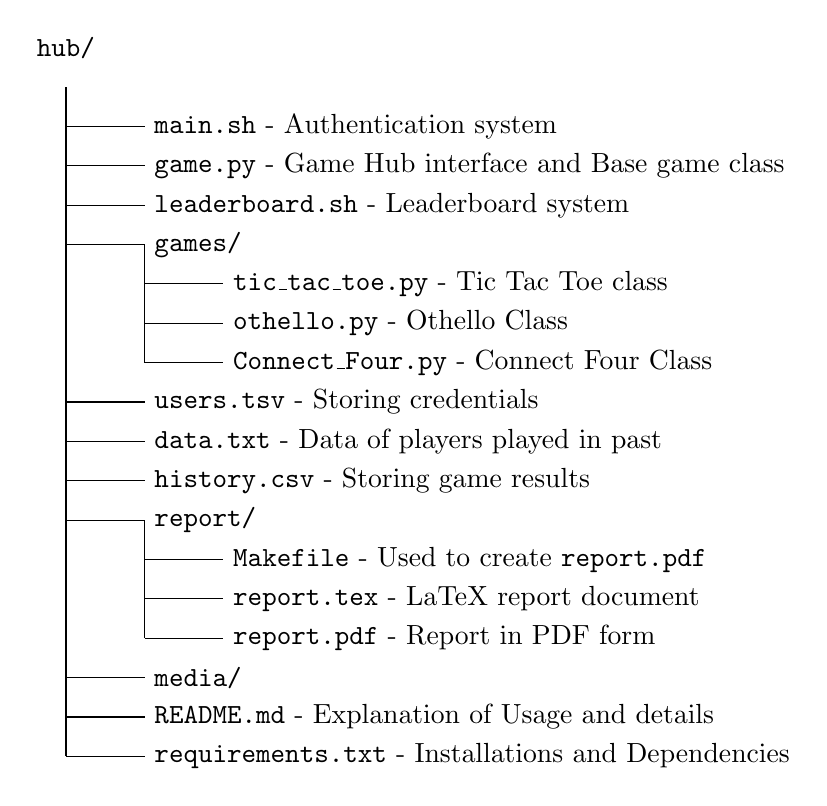
\begin{tikzpicture}[x=1cm, y=1cm]

\node at (0,0) {\texttt{hub/}};
\draw (0,-0.5) -- (0,-9.0); 
\draw (0,-1) -- (1,-1) node[right] {\texttt{main.sh} - Authentication system};
\draw (0,-1.5) -- (1,-1.5) node[right] {\texttt{game.py} - Game Hub interface and Base game class};
\draw (0,-2) -- (1,-2) node[right] {\texttt{leaderboard.sh} - Leaderboard system};
\draw (0,-2.5) -- (1,-2.5) node[right] {\texttt{games/}};

\draw (0,-4.5) -- (1,-4.5) node[right] {\texttt{users.tsv} - Storing credentials};
\draw (0,-5) -- (1,-5) node[right] {\texttt{data.txt} - Data of players played in past}; 
\draw (0,-5.5) -- (1,-5.5) node[right] {\texttt{history.csv} - Storing game results};
\draw (0,-6.0) -- (1,-6.0) node[right] {\texttt{report/}};
\draw (0,-8.0) -- (1,-8.0) node[right] {\texttt{media/}};
\draw (0,-8.5) -- (1,-8.5) node[right] {\texttt{README.md} - Explanation of Usage and details};
\draw (0,-9.0) -- (1,-9.0) node[right] {\texttt{requirements.txt} - Installations and Dependencies};

\draw (1,-2.5) -- (1,-4); 
\draw (1,-6.0) -- (1,-7.5); 
\draw (1,-6.5) -- (2,-6.5) node[right] {\texttt{Makefile} - Used to create \texttt{report.pdf}};
\draw (1,-7.0) -- (2,-7.0) node[right] {\texttt{report.tex} - LaTeX report document};
\draw (1,-7.5) -- (2,-7.5) node[right] {\texttt{report.pdf} - Report in PDF form};
\draw (1,-3) -- (2,-3) node[right] {\texttt{tic\_tac\_toe.py} - Tic Tac Toe class};
\draw (1,-3.5) -- (2,-3.5) node[right] {\texttt{othello.py} - Othello Class};
\draw (1,-4) -- (2,-4) node[right] {\texttt{Connect\_Four.py} - Connect Four Class};

\end{tikzpicture}
\section{Installation and Setup}

This section explains how to install the required dependencies and set up the project for execution.

\subsection{Clone the Repository}
First, clone the project repository and navigate into the project folder:

\begin{verbatim}
git clone <repository-url>
cd hub
\end{verbatim}

\subsection{Install Python Dependencies}
Install all required Python libraries using pip:

\begin{verbatim}
pip install -r requirements.txt
\end{verbatim}

\subsection{Install LaTeX Dependencies (for report compilation)}
To compile the report, install a LaTeX distribution.

On Ubuntu/Debian systems:
\begin{verbatim}
sudo apt install texlive-latex-recommended texlive-latex-extra
\end{verbatim}

On Windows, install MikTeX and ensure pdflatex is added to PATH.

\subsection{Makefile Setup}
Ensure \texttt{make} is installed:

\begin{verbatim}
sudo apt install make
\end{verbatim}

Hopefully this is enough to get the project running.

\section{Usage}

This section explains how to run and interact with the project.

\subsection{Starting the Game Hub}
Run the project using the following command:

\begin{verbatim}
bash main.sh
\end{verbatim}

This launches the authentication system.

\subsection{Login and Registration}
\begin{itemize}
    \item Enter username and password for Player 1 and Player 2
    \item If the user already exists, login is performed using SHA-256 password verification
    \item If the user does not exist, registration is offered
\end{itemize}

After successful authentication, the game engine starts automatically.

\subsection{Game Selection}
A Pygame window opens with a menu where players can choose one of the following games:
\begin{itemize}
    \item Tic-Tac-Toe
    \item Othello
    \item Connect Four
    \item Pop it
\end{itemize}

Players interact using mouse clicks.

\subsection{Gameplay}
\begin{itemize}
    \item Players take alternate turns
    \item The game ends when a win condition or draw condition is reached
\end{itemize}

\subsection{After Each Game}
After completion:
\begin{itemize}
    \item Result is stored in \texttt{history.csv}
    \item A Pygame window showing the username of winner is displayed
    \item The same window will ask for sorting options of leaderboard
    \item Leaderboard is displayed (via leaderboard.sh)
    \item Graphs are shown using Matplotlib
    \item Players can choose to play again or exit
\end{itemize}


\section{Code Design}

\subsection{Authentication System -- \texttt{main.sh}}
The authentication system is implemented using a Bash script that handles both login and registration (hence the function is named \texttt{LorR}) for two players before starting the game.

\paragraph{Login:}
The system prompts each player to enter a username and makes sure that the usernames are valid (non-empty and distinct). If a username already exists in the \texttt{users.tsv} file, the user is asked to enter their password. The entered password is hashed using the SHA-256 algorithm and compared with the stored hashed value in \texttt{users.tsv} to verify the credentials. If the password is incorrect, the user is prompted to verify their username and try again.

\paragraph{Registration:}
If the username does not exist, the system provides an option to register. During registration, the user is required to enter and confirm their password. Once the passwords match, the password is hashed and stored along with the username in the \texttt{users.tsv} file.
After successful authentication of both players, their usernames are passed as command-line arguments to the \texttt{game.py} file, which then starts the game hub.

\subsection{Base Game Class}
A generic class was implemented to represent a two-player board game. Code contains an initiator function and a turn switching function. The players get assigned with player 1 or 2 status and board(using numpy) gets initialized . Turn switching function is self-explanatory 

\subsection{Tic-Tac-Toe Game}
A Tic-Tac-Toe class is created that inherits from the base class. Pygame is used for UI of the game. Board is represented using a 10x10 NumPy array, where each cell stores the state of the position(empty , player1, or player2).
\paragraph{Move Validation:}
Move validation is straightforward, as a move is allowed only if the selected cell is empty.
\paragraph{Win condition:}
The game checks for win after every move. This is done using a function checkwin which checks for a consecutive 5 X or O's in all directions using recursion and slicing methods.

\subsection{Othello Game}
Othello class is created that inherits from the base class. Pygame is used for UI of the game. Board is represented using a 8x8 NumPy array, where each cell stores the state of the position(empty , player1, or player2).
\paragraph{Move validation:}
The \texttt{valid move} function checks whether placing a disc at a given position results in flipping of atleast one opponent disc by going in all 8 directions from the selected cell. A move is considered valid if there exists at least one direction where a continuous sequence of opponent discs is followed by a disc of the current player.

\paragraph{Win Condition:}
Win condition has two stages. After each move, a function is called which checks if all the cells are filled or not. If filled, then using Numpy's sum operation over the board, it will report the winner (or maybe a tie situation). If board is not filled, then we come out of the function and proceed to next stage where valid move availability is checked for the next player using a \texttt{has\_valid\_moves} function. If current player has no valid moves, their turn is skipped.

However, if both players consecutively have no valid moves, the game is ended. And then winner is evaluated by using Numpy's sum operator over the board.

\subsection{Connect Four Game}
Connect Four class is created which inherits from the same base class. Pygame is used for the UI of the game. Board is represented with a 7x7 NumPy array. Players select a column using mouse input, and the piece is placed in the lowest available row within that column.
\paragraph{Move Validation:}
Move validation is handled by checking whether the top-most cell of a column is empty or not. If it is not empty, the column is considered full and the move is not valid.

After a valid move, the correct row is determined by scanning upward from bottom of the column until an empty position is found. Drop animation is implemented using Pygame, where the piece visually falls from the top to its final position.
\paragraph{Win Condition:}
The win condition is evaluated after each move using a recursion and slicing approach similar to the Tic-Tac-Toe game. A helper function \texttt{check\_win()} is used to check for four consecutive X or O in horizontal, vertical, and diagonal directions. If the function returns true, the game is stopped and a win screen is shown indicating which player won.

If the board becomes completely filled without any player achieving four in a row, the game ends in a draw.
\subsection{Pop It Game}
The Pop It game is the latest addition to the hub, inheriting from the base class. It features a grid of "bubbles" where players take turns popping one or more bubbles in a single row. The logic utilizes the base class's dual-side highlighting to track the intense back-and-forth gameplay, ending when the last bubble is popped.
\subsection{Leaderboard System:}
The leaderboard system is implemented using a Bash script that processes the \texttt{history.csv} file to display player performance stats for each game.
The script reads the CSV file and filters entries based on the game name (Tic-Tac-Toe, Othello, or Connect Four). For each game, it calculates the number of wins and losses for every player by counting how many times a player appears as a winner and as a loser in the csv file. Games which end up in tie are not added to the csv file so every line in the csv file has a winner and a loser.
\paragraph{Win/Loss Ratio:}
Using the computed counts, the win/loss ratio is calculated for each player. If a player has zero losses, the ratio is taken equal to the number of wins to avoid division by zero. The results are then formatted into a structured table displaying name, wins, losses and win/loss ratio.
\paragraph{Sorting:}
The leaderboard can be sorted based on different metrics such as wins, losses, or win/loss ratio (using the sort command). This is controlled through a command-line argument passed to the leaderboard.sh from pygame interface.The pygame interface asks for the sort option after each game. Separate leaderboards are generated for each game to allow independent analysis of performance.

\subsection{Data Visualization code}
To provide a visual summary of game statistics, charts are generated using data from \texttt{data.txt} file.

The file is read line by line, and relevant information such as the winner and game name is extracted. A dictionary is used to count the total number of wins for each player, while another dictionary keeps track of how many times each game has been played.
\paragraph{Top players by Wins:}
The players are sorted based on their total number of wins, and the top five players are selected. A bar graph is then plotted to display the number of wins for these players, providing a clear comparison of their performance.
\paragraph{Top players by Wins/Loss Ratio}
The players are sorted based on their win/loss ratio, and the top five players are selected. A bar graph is then plotted to display the ratio values for these players, providing a clear comparison of their performance.
\paragraph{Game Distribution:}
The frequency of each game is used to generate a pie chart, showing the distribution of games played which helps in visualizing which games are played more frequently.

All charts are displayed together (subplots) using \texttt{matplotlib}, with appropriate labels and titles for clarity.
\section{Hurdles Faced}
\begin{itemize}
    \item Adding animations to each game 
    \item Writing win conditions without for loops
    \item Matching themes across all the games (visual consistency)
    \item Finding apt images for background and drawing suitable boards for each game
\end{itemize}
\section{If given more time}
With additional time:
\begin{itemize}
    \item Add sound effects
    \item Add animation effects to Othello
    \item Refine Visual consistency
    \item Optimising Computer mode and implementing it
\end{itemize}
\vfill

\section{Bibliography}
\begin{itemize}
    \item \url{http://docs.python.org/3/tutorial/classes.html}
    \item \url{http://pyga.me}
    \item \url{http://worldothello.org}
    \item \url{http://boardgamegeek.com/boardgame/2719/connect-four}
    \item \url{https://www.w3schools.com/python/numpy/default.asp}
    \item \url{https://www.w3schools.com/python/matplotlib_intro.asp}
\end{itemize}

\end{document}
